\documentclass[class=article, crop=false]{standalone}
\usepackage{my_preamble}
\begin{document}
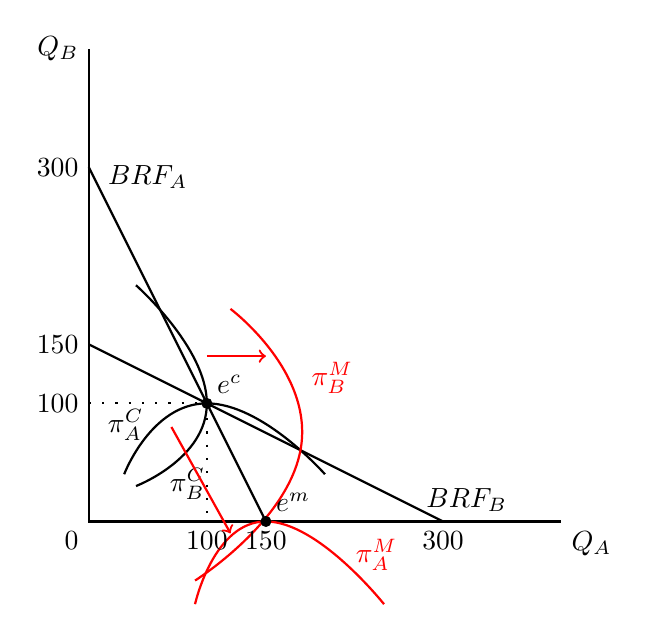
\begin{tikzpicture}[thick,font=\sffamily,scale=1.5]
	%axis
	 \draw (0,4) node[left]{$Q_{B}$} -- (0,0) node[below left] {$0$} 
	  -- (4,0) node[below right]{$Q_{A}$};
	  
	 %BRFs
	\draw[] (0,3) -- (1.5,0); %BRF A
	\draw[] (0,1.5) -- (3,0); %BRF B

	%Iso-profits
	\draw[] plot [smooth, tension=1] coordinates {(0.3,0.4) (1,1) (2,0.4)}; %A's iso-profit 1
	\draw[red] plot [smooth, tension=1] coordinates {(0.9,-0.7) (1.5,0) (2.5,-0.7)}; %A's iso-profit 2
	\draw[] plot [smooth, tension=1] coordinates {(0.4,0.3) (1,1) (0.4,2)}; %B's iso-profit 1
	\draw[red] plot [smooth, tension=1] coordinates {(0.9,-0.5) (1.8,0.65) (1.2,1.8)}; %B's iso-profit 2
	
	%collusion
	%\draw[] (0.46,0.72) -- (0.75,0.5); %Contract curve	
	%\draw[] plot [smooth, tension=1] coordinates {(0.375,0.225) (1.05,0.84) (2,0.225)}; %A's iso-profit collusion
	%\draw[] plot [smooth, tension=1] coordinates {(0.26,0.35) (0.82,1.14) (0.225,2.025)}; %B's iso-profit collusion
	
	%labels
	\node[below] at (0.5,3.1) {$BRF_{A}$}; %BRF A label
	\node[above] at (3.2,0) {$BRF_{B}$}; %BRF B label
	\node[below] at (1.5,0) {$150$}; %A's monopoly quantity
	\node[left] at (0,1.5) {$150$}; %B's monopoly quantity
	\node[below] at (3,0) {$300$}; %PC quantity - A's???
	\node[left] at (0,3) {$300$}; %PC quantity
	\node[above left]at (0.55,0.6) {$\pi_A^C$}; %A's iso-profit 1 label
	\node[above right]at (0.6,0.1) {$\pi_B^C$}; %B's iso-profit 1 label
	\node[above left, red]at (2.7,-0.5) {$\pi_A^M$}; %A's iso-profit 2 label
	\node[above right, red]at (1.8,1) {$\pi_B^M$}; %B's iso-profit 2 label
	
	
	%equilibria labels
	\node[style={fill=black,circle,inner sep=0pt,minimum size=4pt}] at (1,1) { };
	\node[above right]at (1,1) {$e^{c}$};
	\node[style={fill=black,circle,inner sep=0pt,minimum size=4pt}] at (1.5,0) { };
	\node[above right]at (1.5,0) {$e^{m}$};
	
	%dotted lines	
	\draw[loosely dotted] (0,1) node[left]{$100$} -| node[pos=0.25,below=3mm] {}
	  (1,0) node[below]{$100$}; %cournot dotted lines
	%\draw[loosely dotted] (0,0.62) node[left]{$\frac{Q^{M}}{2}$} -| node[pos=0.25,below=3mm] {} (0.62,0) node[below]{$\frac{Q^{M}}{2}$}; %stackelberg dotted lines	
	
	%arrows
	\draw [->, red] (0.7,0.8) -- (1.2,-0.1); %A's arrow
	\draw [->, red] (1,1.4) -- (1.5,1.4); %B's arrow
	%\draw [->] (0.87,1.5) -- (1.17,1.5); %B's arrow
	%\draw [->] (2.1,0.4) -- (2.1,0.25); %A's arrow
\end{tikzpicture}
\end{document}